\section{Förstudie}\label{sec:prestudy}

Detta kapitel redogör för de tekniker, bibliotek, tillvägagångssätt och tidigare befintliga lösningar som identifierats under förstudien och som används för att bidra med en lösning på detta problem.
Syftet med förstudien är att identifiera problem och relevanta tekniska lösningar för att kunna lösa problemet och besvara forskningsfrågorna.

\subsection{Analys av möjliga lösningar}
Under förstudien identifierades ett antal tekniker och tillvägagångssätt som kommer att användas för att lösa problemet med ineffektiv informationshantering.

\subsubsection{API-baserad lösning}

Ett möjligt sätt för att ge en LLM tillgång till organisationens information är att skapa en lösning som direkt exponerar de befintliga systemens API:er som verktyg.
LLM:en tolkar då användarens fråga och avgör själv vilket eller vilka verktyg som ska anropas för att hämta information från rätt system.
Denna lösning introducerar inget extra datalager och kräver ingen omstrukturering av befintlig data, utan nyttjar endast de API:er som redan finns.

Det är dock viktigt att ta hänsyn till att denna lösning i grunden inte förändrar hur data är strukturerad eller representerad.
Information förblir spridd över separata system utan gemensam semantisk kontext, och LLM:en bär hela ansvaret för att koppla samman information från de olika källorna.
Denna lösning inkluderas i arbetet primärt som en jämförelsepunkt mot den grafbaserade lösningen, för att undersöka om en grafbaserad lösning faktiskt ger LLM:en fördelar att koppla samman information från olika källor.


\subsubsection{Grafbaserad lösning}

Ett identifierat angreppssätt för att ge en LLM tillgång till organisationens information är att skapa en kunskapsgraf innehållande data och information från de olika interna systemen.
Data från de olika systemen samlas under en gemensam struktur där samband och relationer mellan dem skapas.

Genom denna representation av data förväntas en LLM kunna koppla samman information från olika källor mer effektivt och därmed kunna navigera relationer med ett enda verktyg istället för att anropa flera olika API:er och själv försöka koppla samman informationen.

Denna lösning bedöms ge färre verktygsanrop vid mer komplexa frågor som kräver tydliga samband mellan data från olika källor, och därmed bidra till en mer effektiv informationshämtning.

\subsubsection{Vector databas / embeddings (RAG)}
En annan potentiell lösning som identifieras under förstudien är att använda en vektordatabas och embeddings för att strukturera och organisera data och information.
Denna lösning bygger på att omvandla användarfrågan till en vektorrepresentation (embedding) och sedan jämföra mot de lagrade vektorerna i databasen för att hitta de mest liknande\cite{1}.

Denna lösning varken implementeras elelr undersöks vidare i detta arbet då den liksom den API-baserade lösningen inte förändrar hur relationer och samband mellan data från olika källor representeras, vilket är det primära syftet med detta arbete.

\subsection{Val av teknisk arkitektur}
Under förstudien identifieras flera olika verktyg och tekniker för att implementera de olika lösningarna på.
Därför beslutas det om vilka specifika tekniker och verktyg som används i den slutgiltiga lösningen.

\subsubsection{Val av grafdatabas}
Grafdatabasens syfte i detta arbete är att lagra data och information från de olika interna systemet i form av en kunskapsgraf.
För att välja vilken grafdatabas som ska användas görs det en undersökning om vilken som lämpar sig bäst specifikt för detta arbete.

Databasen som väljs är Neo4j. Detta val görs då det är en marknasledande grafdatabas med stor användarbas och bra community-stöd.
Den har en låg inlärningströskel med omfattande dokumentation och många guider för att komma igång. Den är även av typen OLAP (Online Analytical Processing), vilket betyder att den är specifikt anpassad för just affärsintelligens och informationssökning vilket är det primära syftet för databasen i detta arbete\cite{17}.

\subsubsection{Val av kommunikationslager}
Kommunikationslagret som väljs till detta arbete är MCP. Detta val görs då det är ett modernt och lättanvänt sätt att låta LLM:er kommunicera med externa system.
Denna lösning väljs framförallt för att den fungerar för båda de lösningarna som jämförs mot varandra (API-baserad och grafbaserad).

\subsubsection{Val av LLM}
För att jämföra de två lösningarna på ett rättvist sätt krävs det att samma LLM används för båda lösningarna. 
Den LLM som används i detta arbete är GPT-5.4-mini. Modellen valdes för att den är kostnadseffektiv med hög prestanda, vilket möjliggör ett stort antal tester utan att kostnaden blir för hög.

Eftersom det ständigt släpps nya AI-modeller är det viktiga i detta arbete inte vilken modell som används utan egentligen bara att samma modell används för båda lösningarna.

\subsection{Design av kunskapsgrafen och grafdatabasen}
Avgränsningarna i kapitel \ref{subsec:scope} gör det inte möjligt att skapa ett komplett system där LLM:en själv hämtar och uppdaterar data i grafdatabasen.
Därför undersöks det hur databasen ska designas för att efterlikna de olika informationskällorna som finns i en verklig organisation.

De informationskällor som inkluderas i grafdatabasen är: Confluence, Slack och Github.
 Dessa informationskällor är tillräckligt många och tillräckligt breda för att kunna erbjuda en realistisk representation av en verklig organisations informationskällor.

De entiteter och relationer som skapas i grafdatabasen är utformade för att efterlikna de olika typer av information som finns i de olika informationskällorna, samt de relationer som finns mellan dem.
De entiteter som inkluderas är: \textit{Person}, \textit{Team}, 
\textit{Project}, \textit{Repository}, \textit{Issue}, \textit{Commit}, 
\textit{SlackChannel}, \textit{Post}, \textit{ConfluenceSpace}
\textit{Document}. Mellan dessa entiteter skapas relationer som exempelvis \textit{WORKS\_ON}, \textit{MEMBER\_OF}, \textit{HAS\_ISSUE}, \textit{HAS\_COMMIT}, \textit{POSTED\_IN}, \textit{CONTAINS}.

Figur \ref{fig:yyy} Visar en komplett bild över relationer mellan noder i grafdatabasen.

\begin{figure}[H]
  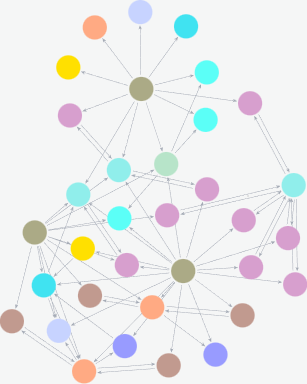
\includegraphics[width=\textwidth]{Figures/kg_quests/yyy.png}
  \caption{Fullständig bild över relationer mellan noder i grafdatabasen}\label{fig:yyy}
\end{figure}

I Figur \ref{fig:labels} visas etiketterna till entiteterna med färgkodningen som används i bilden ovan.

\begin{figure}[H]
  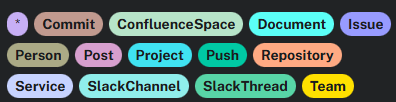
\includegraphics[width=\textwidth]{Figures/labels.png}
  \caption{Etiketterna till entiteterna i grafdatabasen}\label{fig:labels}
\end{figure}

\subsection{Design av API-baserade lösningen}
För att täcka samma informationskällor som kunskapsgrafen identifieras att verktyg behövs för att kommunicera med API:er från Confluence, Slack och GitHub.
Exempel på verktyg som identifieras är ett som hämtar alla personer i ett GitHub-repository, alla meddelanden i en Slack-kanal, eller alla dokument skapade av en viss person i Confluence.

\subsection{Design av frågor}

Det beslutas att utvärderingen ska baseras på 15 testfrågor fördelade över tre komplexitetsnivåer.
De simpla frågorna (Q1–Q5) kräver ingen koppling mellan datakällor och kan besvaras med ett enda anrop till en källa.
De medelsvåra frågorna (Q6–Q10) kräver antingen flera anrop till samma datakälla eller like mer avancerat resonemang för att nå svaret.
De komplexa frågorna (Q11–Q15) kräver ofta kopplingar mellan data från olika källor, vilket är det scenario där skillnaden mellan de två lösningarna förväntas vara som störst.
De fullständiga frågorna presenteras i kapitel \ref{subsec:questTest}.

\subsection{Utvärderingsstrategi (Koppling till mål)}

Under förstudien identifieras hur utvärderingen av de två lösningarna skulle
  utformas för att kunna besvara de verifierbara målen i kapitel
  \ref{subsec:researchquestion}.

För varje identifierbart mål identifieras ett konkret mätvärde:

  \begin{itemize}
    \item \textbf{Effektivitet} — svarstid i millisekunder är ett objektivt och
    enkelt mätbart mått på hur snabbt systemet hämtar information.

    \item \textbf{Kvalitet på svar} — korrekthet bedömd manuellt mot ett
    förväntat svar.

    \item \textbf{Resursanvändning} — antal verktygsanrop speglar hur effektivt
    LLM:en navigerar till rätt information, och är ett direkt mått på hur
    väl informationsrepresentationen stödjer LLM:ens resonemang.

  \end{itemize}

\subsection{Sammanfattning av designbeslut}

Förstudien resulterar i ett antal konkreta beslut som tillsammans utgör
grunden för implementationen och utvärderingen i detta arbete.

Av de tre identifierade lösningsalternativen väljs två att implementeras:
den grafbaserade lösningen som arbetets huvudsakliga fokus, samt
den API-baserade lösningen som jämförelsepunkt. Den vektorbaserade
(RAG) lösningen utesluts då den inte består av relationsstrukturen mellan
data, vilket är det arbetet syftar till att undersöka.

Som teknisk grund väljs Neo4j som grafdatabas tack vare dess användarvänlighet och dokumentationsstöd, MCP som kommunikationslager för att på ett enhetligt
sätt exponera verktyg för båda lösningarna, samt GPT-5.4-mini som LLM.

Kunskapsgrafen och den API-baserade lösningen designas för att täcka
samma informationskällor och därigenom möjliggöra en rättvis jämförelse.

Testfrågorna utformas i tre komplexitetsnivåer för att undersöka i vilka situationer de två lösningarna
skiljer sig åt, med fokus på de komplexa frågorna där det krävs kopplingar mellan data från olika källor.

Utvärderingen baseras på tre mätvärden som är svarstid, antal verktygsanrop
och korrekthet, som direkt kopplar till de verifierbara målen i kapitel
\ref{subsec:researchquestion}.


